\documentclass[11pt,singlecolumn]{scrartcl}
\usepackage[masterthesis]{systems-cover}
\usepackage{amsmath,amssymb,amstext}
\usepackage[utf8]{inputenc}
\usepackage[english]{babel}
\usepackage{fancyhdr}
\usepackage{graphicx}
\usepackage[capposition=bottom]{floatrow}
\usepackage{listings}


\lstset{frame=tb,
  language=Java,
  aboveskip=3mm,
  belowskip=3mm,
  showstringspaces=false,
  columns=flexible,
  basicstyle={\small\ttfamily},
  numbers=left,
  numberstyle=\tiny,
  breaklines=true,
  breakatwhitespace=true,
  tabsize=3
}

\pagestyle{fancy}
\fancyhf{}
\fancyhead[LE,RO]{A High-level Graph Query Language Interface for Differential Dataflow}
\fancyhead[RE,LO]{Lukas Striebel}

\fancyfoot[RE,lO]{Master Thesis}
\fancyfoot[LE,RO]{\thepage}

\renewcommand{\headrulewidth}{2pt}
\renewcommand{\footrulewidth}{1pt}

\covernum{164}
\covertitle{A High-level Graph Query Language Interface for Differential Dataflow}
\coverauthor{Lukas Striebel}
\coverdate{October 2016 - April 2017}
\coversupervisedby{Prof.\ Timothy Roscoe\\Dr. Ioannis Liagouris\\Dr. Desislava Demitrova\\Moritz Hoffmann}


\begin{document}

\hspace{60mm}
\begin{center}
 \textbf{Abstract} \end{center}
In today's business world, Social Networks have become one of the most important if not the most important platforms to advertise your product and gain new customers. Graph databases have been increasing in popularity in comparison to traditional relational databases. This tendency has given birth to the need of powerful and graph datawarehouses and query evaluators. Thus, we present cool program.


\clearpage
\tableofcontents
\clearpage
\section{Introduction}
\subsection{Motivation}
\subsection{Structure of the Thesis}
The Thesis has the following layout:\\
First, we give an overview of the technologies used in the Thesis.\\
We continue by giving a detailed explanation of the query parser and query evaluator. Next, we describe the experiments that were run in order to determine the performance of the program. Finally, we draw our conclusion and show potential future work.
\clearpage

\section{Background}
In this section, all the relevant technologies used in the Thesis are explained.
\subsection{The Property Graph Query Language}

The Property Graph Query Language (PGQL) was developed by Oskar van Rest at Oracle. \cite{vanRest:2016} PGQL enables developers to write intuitive path queries over a property graph. A PGQL query consists of 4 clauses, two of them are optional.
\begin{itemize} 
\item Path Clause (optional)
\item Select Clause (required)
\item Where Clause (required)
\item Solution Modifier Clause (optional)
\end{itemize}

In the Path Clause custom path patterns are defined, which are to be used again in the Where Clause.\\
\textbf{Example:}\\
\begin{lstlisting}
PATH connects_to := (:Generator) -[:has_connector]-> (:Connector WITH status = 'OPERATIVE') <-[:has_connector]- (:Generator)
 \end{lstlisting}
The Select Clause bears great similarity to the SQL one. Here, the set of properties one wishes to retrieve is defined. Possible Selections are either\\
\begin{itemize} 
\item everything, indicated by the use of * 
\item certain attributes of edges and/or vertices
\item Aggregation of certain attributes of edges and/or vertices.
\end{itemize}
 Currently, there are five types of aggregations supported:\\
 \begin{itemize} 
\item COUNT, returns the number of tuples in the solution 
\item MAX, returns the maximum value of an attribute in any tuple. The specified attribute has to be numeric.
\item MIN, returns the minimum value of an attribute in any tuple. The specified attribute has to be numeric.
\item SUM, returns the sum of an attribute over all the tuples. The specified attribute has to be numeric.
\item AVG, returns the average of an attribute over all the tuple. The specified attribute has to be numeric.
\end{itemize}
\textbf{Example:}\\
\begin{lstlisting}
SELECT v.name, AVG(v.age)
 \end{lstlisting} 
The most complex part of the query is the Where Clause. In this section, all the requirements that the edges and vertices of the result set have to fulfill are specified.
\textbf{Example:}\\
\begin{verbatim}
  WHERE v.name = 'Alice', v.age > 30
\end{verbatim}

\clearpage
\subsection{Dataflow Computation}
Dataflow oriented computation is a young field in Computer Science.

\clearpage

\subsection{Differential Dataflow}

Differential Dataflow was developed by Frank McSherry at Microsoft. \cite{Differential}
Rather than rewriting the entire data every time a change occurs, Differential Dataflow only keeps track of the changes made to the data. This allows for huge timesavings when executing the same operation multiple times on different data, since the results of previous computations can be reused.
\clearpage

\subsection{The Rust Programming Language}
Rust is a fairly new programming language. It's origin lies with the Mozilla Company, where former employee Graydon Hoare started development in 2006. In the 2009, Mozilla offically began sponsering th eproject.\\
Rust has been praised as it combines . The Rust compiler is self-hosted, meaning it is written in Rust as well. Rust won the Award for Most Loved Programming Language in 2016, host by the Stack Overflow Community.
Rust is completly opensource, and a big part of the code was written by members of the community.
\clearpage

\section{Parser}
In the following, we describe how our parser is build. The Parser is build using nom, \cite {Nom}. Nom was developed by Geoffroy Couprie. It is a byte oriented, zero copy, streaming Parser Library written in Rust. The library provides macros, functions and enums which faciliate the parsing process.\\\\
The most commonly used macros were:
\begin{itemize} 
\item do\_parse!: Takes a list of parsers as inputs and applies them sequentially, finally returns a tupel.
\item alt\_complete!: Takes a set of parsers as input and applies them until one succeeds. Returns the result of the first successful parser.
\item opt!: Takes a parsers as input and makes it optional. Returns None if parser was unsuccessful or Some otherwise.
\item tag!: Parses a specific String. Aborts if the String is not found.
\item named!: Faciliates the creation of new custom parsers.
\item many0!: Applies the parser 0 or more times.
\item many1!: Applies the parser 1 or more times. 
\end{itemize}

As mentioned in Section 2.1, the Parser has to recognize the following 4 clauses: Path definitions, select, where, solution modifier.
\\The main parse function therefore looks:
\begin{lstlisting}
named!(pgql_query<Query>,
    do_parse!(
	paths: opt!(paths) >>
	space >>
	select: select_clause >>
        space >>
        vvhere: where_clause >>
	space >>
        solmod: opt!(solutionModifier) >>
        (Query { select: select, vvhere: vvhere, paths: paths, solmod: solmod})
 \end{lstlisting} 
\clearpage

\subsection{Path Clause}

The Path Clause is a list of definitions. Each Path definition starts with a name, followed by `:=' and then a path description. The path defined in this clause can then be reused in the Where Clause. One of many difficulties encountered while writing the parser, is the ability to differentiate between a single path definition and multiple ones, seperated by commas.


\clearpage
\subsection{Select Clause}
The Select Clause of PGQL is very similar to the SQL one. Started by the keyword `Select', a list of attributes is provided. Attributes may be renamed with the keyword `as'. Aggregate functions like `Sum', `Avg' etc. may also be accessed.

\clearpage

\subsection{Where Clause}
The Where Clause consists of a list of Constraints. Each constraint defines either a path or value requirement that has to be fulfilled by the respective vertex or edge.
 
 \subsubsection{Path Constraints}
 Path Constraints are patterns, which are matched against the graph. If a set vertices does not fit the pattern, it is discarded.\\
 A typical Path Constraint requires a vertex to have certain edges to other vertices. For example, the constraint: (v) -> (u) requires that the vertex v has a direct edge to the vertex v.
 
 \subsubsection{Value Constraints}
 Value Constraints are constraints on attributes of the Vertex, e.g. name = `Alice' or age \textless  40. Every Value Constraint has to include one or multiple vertex attributes, and one or more Literals. Literals are raw values, and come in 3 types:
 \begin{itemize} 
\item Strings e.g. `Alice'
\item Floats e.g. 40
\item Booleans, which are either true or false
\end{itemize}
 
 \begin{lstlisting}
pub enum Literal {
    Str(String),
    Float(f32),
    Boolean(bool),
} 
 
named!(literal<Literal>,
    alt_complete!(
        float       => { |f| Literal::Float(f)             } |
        boolean     => { |b| Literal::Boolean(b)           } |
        string      => { |s| Literal::Str(String::from(s)) } 
            
    )
);
 \end{lstlisting}
 
 \clearpage
 
 \subsection{Solution Modifier Clause}
 
 The Solution Modifier Clause consists of three parts: 
  \begin{itemize} 
\item GroupBy Clause
\item OrderClause
\item Offset and Limit Clause
\end{itemize}
 All clauses are optional and can be omitted. 
 
\clearpage



\section{Query Evaluation}

\subsection{Graph Loader}
The Loading of the graph plays a major part of the entire program execution time. To load a graph from a text file into differntial Dataflow, an entirely new parser had to be written. This parser was also built using nom. In order fo it to properly recognize a graph, the graph has to be supplied in the Vertex-Edge-List format. This format gives us a text file (.txt), which contains two lists. First, all the vertices and their attributes are described. The vertices are ordered ascing according to their ID. The IDs have to start at 1 and must be continuous.
\subsection{Construction of the Dataflow}

\clearpage



\section{Benchmarking}
All experiments were run on server. The machine contained 48 Amd cores. The installed memory was 128 GB of RAM.\\
In the experiment, four different topologies were used:\\
\textbf{Large Fattree}  The large fattree topology is the largest one of the four topologies. It contains 55'000 vertices, of which 2'880 are switches. Furthermore the graph posses a total of 50'000 bidirectional edges. Since one bidirectional edge is represented by two directed edges, there are a total of 100'000 edges in the collection.\\\\
\textbf{Small Fattree}  The large fattree topology is the largest one of the four topologies. It contains 55'000 vertices, of which 2'880 are switches. Furthermore the graph posses a total of 50'000 bidirectional edges. Since one bidirectional edge is represented by two directed edges, there are a total of 100'000 edges in the collection.\\\\
\textbf{Large Jellyfish}  The large fattree topology is the largest one of the four topologies. It contains 55'000 vertices, of which 2'880 are switches. Furthermore the graph posses a total of 50'000 bidirectional edges. Since one bidirectional edge is represented by two directed edges, there are a total of 100'000 edges in the collection.\\\\
\textbf{Small Jellyfish}  The large fattree topology is the largest one of the four topologies. It contains 55'000 vertices, of which 2'880 are switches. Furthermore the graph posses a total of 50'000 bidirectional edges. Since one bidirectional edge is represented by two directed edges, there are a total of 100'000 edges in the collection.
\clearpage


\section{Results and Discussion}
\textbf{Things to consider}\\\\
1. Weight is an attribute of the edges and (as far as I know) uniformly distributed from 1 to 9. The selection weight \textless 2 will therefore remove around 90\% of all edges., which speeds up the join process immensely.\\\\
2. Since Timely does not like HashMaps at all, attributes of vertices and edges are store in a Vector of (String, Literal) tuples. However, in order to do a selection, this Vector has to be transformed back into a HashMap, which takes some time. Therefore  the more selection a query contains, the slower it should be.\\\\
3. One Edge in the query triggers two joins in the evaluation,  because we have to join the edge collection twice with the vertex collection.\\\\
4. These are the results of the large fattree, with nearly 60'000 vertices and 50'000 bidirectional edge (ergo 100'000 in the collection). The results look very similar for the smaller fattree topology, just a bit smaller in magnitude.\\\\
\textbf{Overview}


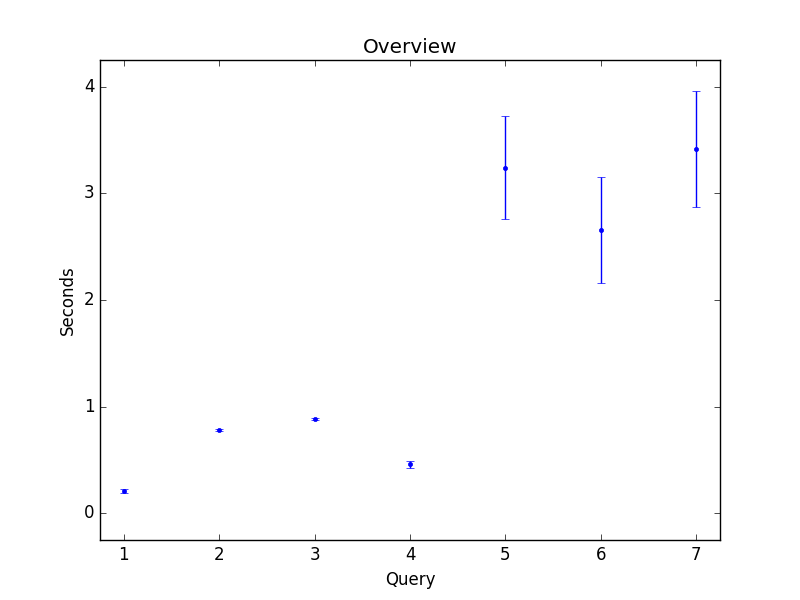
\includegraphics[width=1\textwidth]{overview}
\clearpage
\textbf{Query 1}\\
\begin{verbatim}
SELECT * WHERE u.label() = 'switch', u.position = 'access'
\end{verbatim}
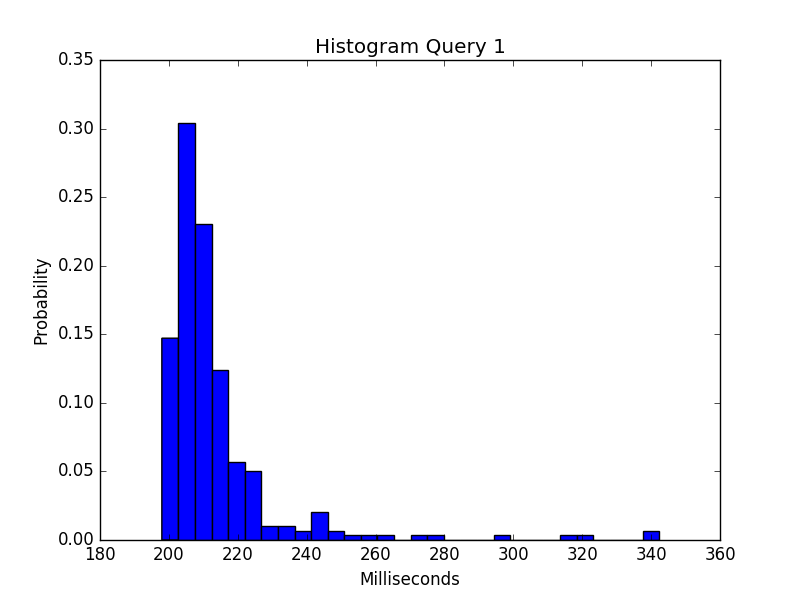
\includegraphics[width=1\textwidth]{q1}
2 simple selections, 0 joins. One pass through the vertices collection is enough to produce the result. 200 milliseconds evaluation time.
\clearpage
\textbf{Query2}\\
\begin{verbatim}
SELECT * WHERE (n) -[e with weight < 4]-> (m)\end{verbatim}
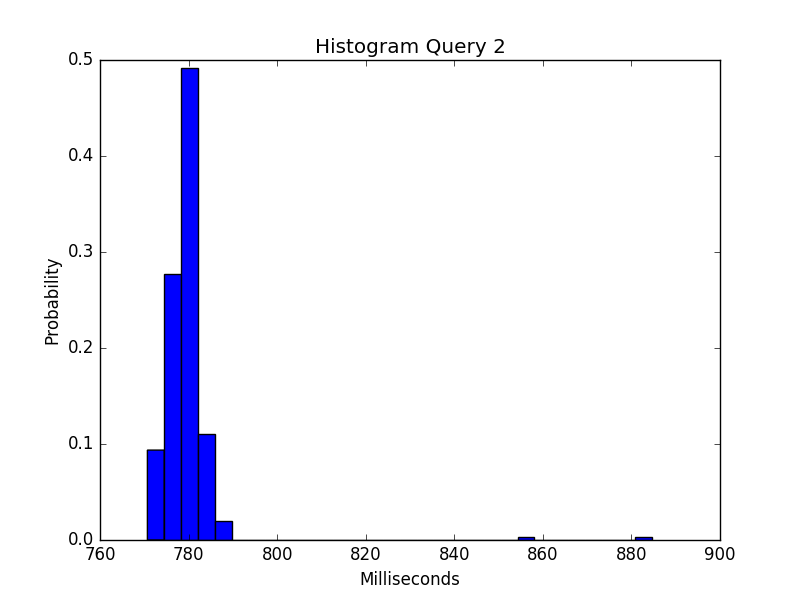
\includegraphics[width=1\textwidth]{q2}
2 Joins and 1 Selection. The joins are not very expensive since we only use about 30\% of the edges. 700 milliseconds evaluation time.
\clearpage
\textbf{Query3}\\
\begin{verbatim}
SELECT * WHERE (n:switch) -> (m with position = 'distribution')\end{verbatim}
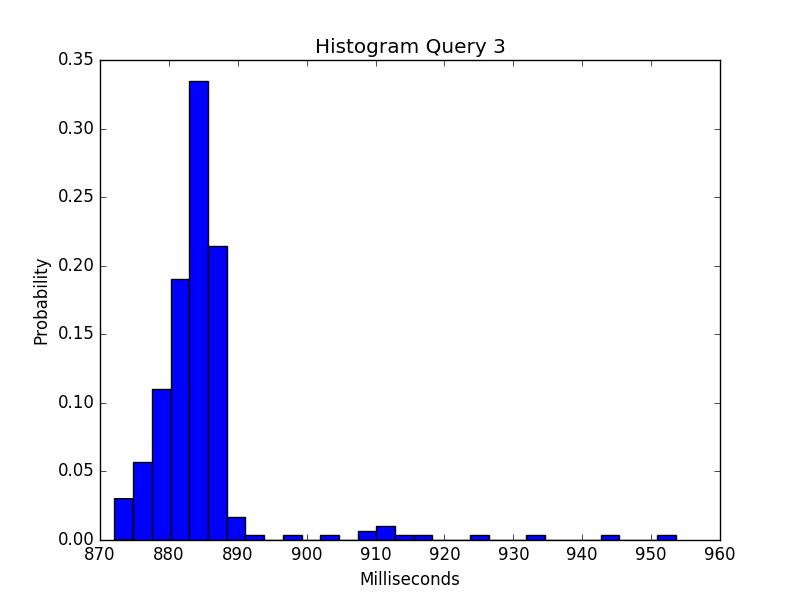
\includegraphics[width=1\textwidth]{q3}
2 Joins and 2 Selections. I expected this query to be a little bit slower since we are using all the edges in the joins, but it is only a tiny bit slower than Query 2.
\clearpage
\textbf{Query4}\\
\begin{verbatim}
SELECT * WHERE (n with position = 'distribution')
-[e with weight > 8]-> (m with position = 'access')\end{verbatim}
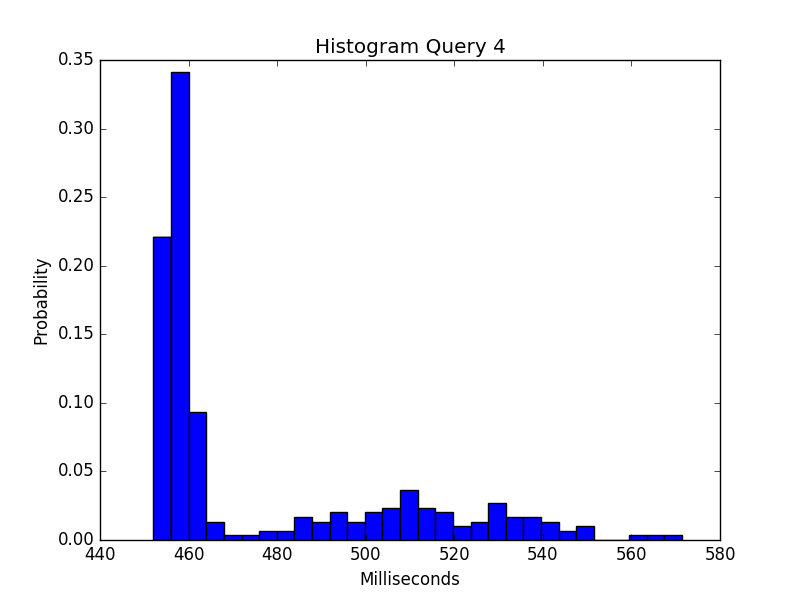
\includegraphics[width=1\textwidth]{q42}
2 Joins and 3 Selections. Even though this query has more constraints than Query 2 and 3, it is faster since we only use 10\% of the edges in the joins. 
\clearpage
\textbf{Query5}\\
\begin{verbatim}
SELECT * WHERE (u WITH position = 'access') -> (v WITH position = 'distribution')
 -> (w WITH position = 'core')\end{verbatim}
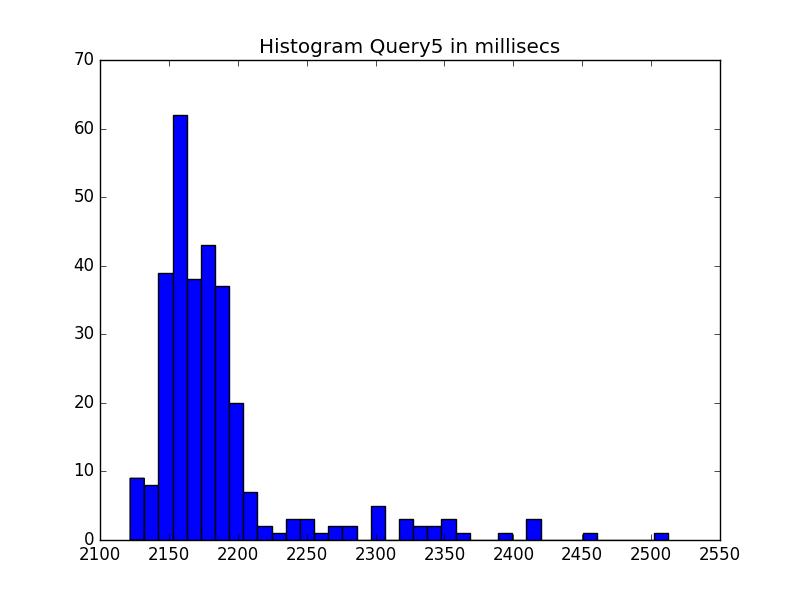
\includegraphics[width=1\textwidth]{q5}
4 Joins and 3 Selections. The last 3 queries all contain multiple query edges and are much slower. Since there is no selection on the edge, this particular query is quite slow even though it has "only" 4 joins.
\clearpage
\textbf{Query6}\\
\begin{verbatim}
SELECT * WHERE (u WITH position = 'access')
 -[e with weight  < 2]-> (v WITH position = 'distribution')
 -[f with weight > 8]-> (w WITH position = 'core')\end{verbatim}
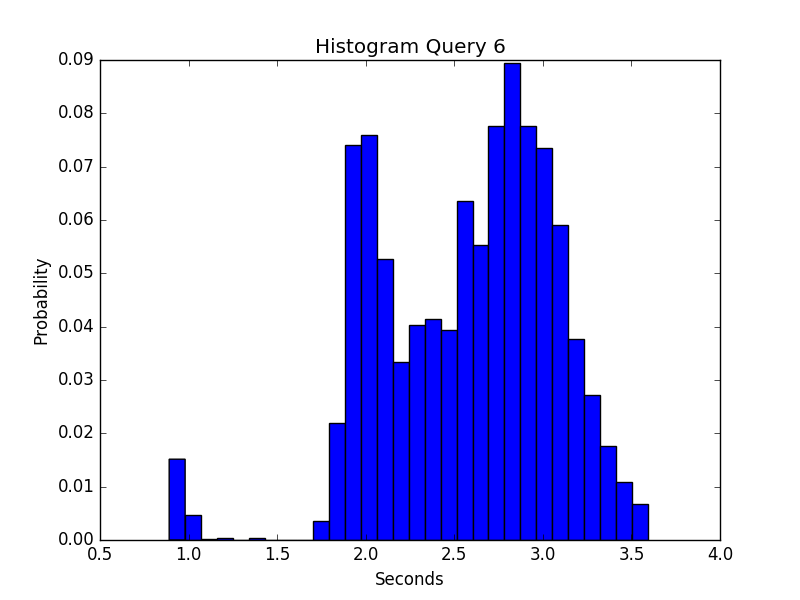
\includegraphics[width=1\textwidth]{q6}
4 Joins and 5 Selections. Like query 4, the evaluation time goes down as we add more constraints on the edges. Since we have a lot less tuples in the 3rd and 4th join, this query is faster than previous one.
\clearpage
\textbf{Query7}\\
\begin{verbatim}
SELECT * WHERE (u WITH position = 'access')
 -[e with weight  < 2]-> (v WITH position = 'distribution')
 -[f with weight  < 2]-> (w WITH position = 'core')
 -[g with weight  < 2]-> (x WITH position = 'distribution')\end{verbatim}
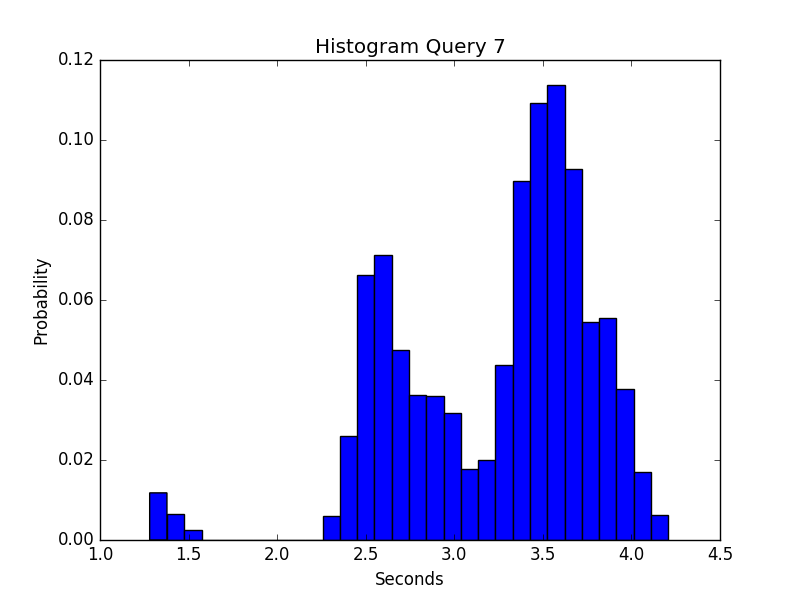
\includegraphics[width=1\textwidth]{q71}
6 Joins and 7 Selections. This is probably the most interesting result. We add two more joins to the query, but we restrict the number of edges used in all the joins dramatically. This consequently leads to a surprisingly low evaluation time, almost on the level as query 5. This demonstrates how big the impact of the joins is for the evaluation time.
\clearpage
\textbf{Query 8}\\
\begin{verbatim}
SELECT * WHERE (u WITH position = 'access') -> (v WITH position = 'distribution')
 -> (w WITH position = 'core') -> (x WITH position = 'distribution')\end{verbatim}
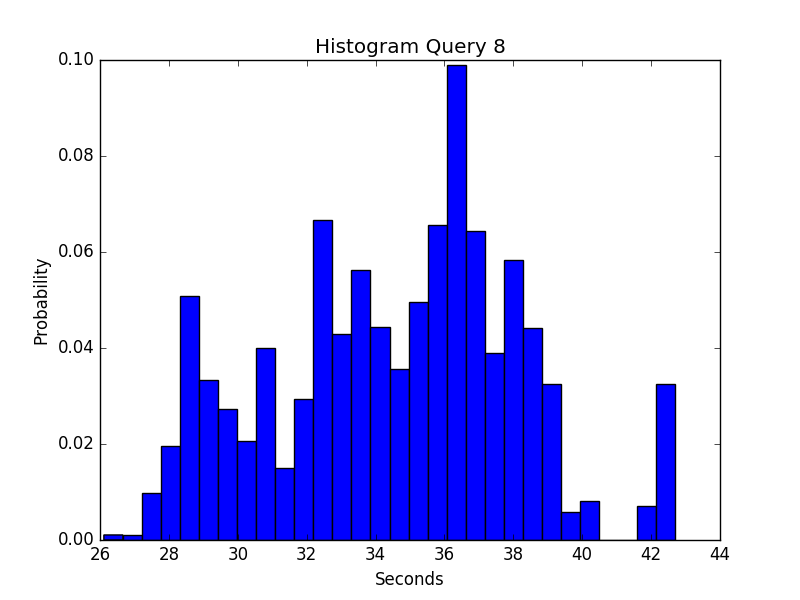
\includegraphics[width=1\textwidth]{q81}
6 Joins and 4 Selections. I have not included this query in the figure because the evaluation times are around 30 to 40 seconds when run with 48 workers. When using only a single worker I have measured evaluation times over 10 minutes. This is due to the fact that we join 6 times with the full edge collection.
\clearpage

\section{Related Work}
In this chapter we give an overview of other existing graph databases and query evluators.

\subsection{PQL}
A program query language, PQL for short, is a source language-independent notation to specify program queries and program views. PQL is used as an interface to Static Program Analyzers (SPA), interactive tools that enhance program understanding by answering queries about programs. Queris on global program design as well as searches for detail code patterns are both possible in PQL. Program queries and patterns supported by other notations described in literature and those supported by commercial tools can be written simply and naturally in PQL.\cite {PQL}

\clearpage

\subsection{Green-Marl}
Green-Marl is a domain-specific language (DSL) with high level language construct that allow developers to describe their graph analysis algorithms intuitively, but expose the data-level parallelism inherent in the algorithms. Green-Marl comes with its own compiler which translates high-level algorithmic description written in Green-Marl into an efficient C++ implementation by exploiting this exposed datalevel parallelism. Furthermore, the Green-Marl compiler applies a set of optimizations that take advantage of the high-level semantic knowledge encoded in the Green-Marl DSL. Most graph analysis algorithms can be written very intuitively with Green-Marl and experimental results show that the compiler-generated implementation out of such descriptions performs just as well as or better than highly-tuned handcoded implementations.\cite {Greenmarl}

\clearpage

\subsection{Gremlin}
Developed by the Apache Software Foundation, Gremlin is a query language as well as a graph traversal machine. The graph traversal machine Gremlin consists of three parts that continously interact with each other: first the graph, second the traversal and finally the set of traversers. The traversers move about the graph according to the instructions specified in the traversal, where the result of the computation is the ultimate locations of all halted traversers. A Gremlin machine can be executed over any supporting graph computing system such as an OLTP graph database and/or an OLAP graph processor. The language Gremlin is a functional language implemented in the user’s native programming language. Gremlin supports both imperative and declarative querying.
\cite{Gremlin}

\clearpage

\subsection{SQLGraph}
SQLGraph is a Graph Store that combines existing relational optimizers with a novel schema, in an attempt to give better performance for property graph storage and retrieval than popular noSQL graph stores. The schema combines relational storage for adjacency information with JSON storage for vertex and edge attributes. This particular schema design has benefits compared to a purely relational or purely JSON solution. The query translation mechanism translates Gremlin queries with no side effects into SQL queries so that one can leverage relational query optimizers. \cite{Sun:2015}

\clearpage

\subsection{GraphiQL}
GRAPHiQL is an intuitive query language for graph analytics, which allows developers to reason in terms of nodes and edges rather than the tables and joins which are used in relational databases. GRAPHiQL provides key graph constructs such as looping, recursion, and neighborhood operations. At runtime, GRAPHiQL compiles graph programs into efficient SQL queries that can run on any relational database. \cite {Graphiql}

\clearpage

\section{Summary}

\subsection{Conclusion}

\subsection{Acknowledgements}
I would like to thank my supervisors John Liagouris, Desislava Dimitrova and Moritz Hoffmann.

\clearpage


\bibliography{MA}{}
\bibliographystyle{plain}
\end{document}
